%
% 13-lie.tex -- Lie-Gruppen
%
% (c) 2022 Prof Dr Andreas Müller, OST Ostschweizer Fachhochschule
%

%
% Lie-Gruppen
%
\subsection{Lie-Gruppen
\label{buch:gruppen:subsection:lie-gruppen}}
Die endlichen Gruppen unterscheiden sich grundlegend von der Gruppe
der Drehwinkel.
In $\mathbb{R}$, $\mathbb{R}/2\pi\mathbb{Z}$, $S^1$ und $\mathbb{C}^*$
steht nicht nur die aus der Gruppenoperation abgeleitete algebraische
Struktur zur Verfügung.

%
% Topologische Gruppen
%
\subsubsection{Topologische Gruppen}
Vielmehr kann man auch von konvergenten Folgen von Gruppenelementen
sprechen und davon, ob eine Abbildung zwischen diesen Gruppen
stetig ist.
Man nennt eine solche Gruppe eine {\em topologische Gruppe}.
\index{topologische Gruppe}%

\begin{beispiel}
Die Menge
\(
\mathbb{Q}^*
=
\mathbb{Q} \setminus\{0\}
\)
ist eine Gruppe mit der Multiplikation als Gruppenoperation.
\end{beispiel}

Die Gruppe $\mathbb{Q}^*$ ist eine topologische Gruppe.
Als Teilmenge von $\mathbb{Q}$ ist klar, was eine Cauchy-Folge in
$\mathbb{Q}^*$ ist.
Es gibt aber auch Cauchy-Folgen in $\mathbb{Q}^*$, die nicht konvergieren.
Die Folge
\[
x_0=1,\;
x_{n+1} = \frac12\biggl(x_n+\frac{2}{x_n}\biggr),\; n\in\mathbb{N},
\]
ist eine Folge von rationalen Zahlen, die gegen einen Fixpunkt der
Funktion
\[
x\mapsto f(x)=\frac12\biggl(x+\frac{2}{x}\biggr)
\]
konvergiert.
Durch Multiplikation mit $x$ findet man
\[
x=f(x)
\quad\Rightarrow\quad
x^2=\frac12 x^2 + 1
\quad\Rightarrow\quad
\frac12x^2=1
\quad\Rightarrow\quad
x^2=2
\quad\Rightarrow\quad
x=\!\sqrt{2},
\]
insbesondere ist der Grenzwert nicht in $\mathbb{Q}^*$.

\begin{definition}
\label{buch:gruppen:gruppe:def:topgruppe}
Eine topologische Gruppe $G$ ist eine Gruppe $G$, deren Verknüpfungsabbildung
$(x,y)\mapsto xy$ und das inverse Element $x\mapsto x^{-1}$ stetig sind.
Für konvergente Folgen $x_n\to x$ und $y_n\to y$ in $G$ gilt dann
\begin{align*}
\lim_{n\to \infty} x_ny_n &= \lim_{n\to\infty} x_n \lim_{n\to\infty} y_n = xy
\\
\lim_{n\to \infty} x_n^{-1} &= (\lim_{n\to\infty} x_n)^{-1} = x^{-1}
\end{align*}
\end{definition}

%
% Koordinatensysteme
%
\subsubsection{Koordinatensysteme}
Für Funktionen auf der Gruppe $\mathbb{R}$ ist sogar die Ableitung
definiert.
Eine solche lässt sich auch für Funktionen auf den Gruppen 
$S^1$ und $\operatorname{SO}(2)$ definieren, indem man diese Gruppen
mit einer geeigneten Parametrisierung beschreibt.
Die der Ableitungsbegriff nur für Funktionen $\mathbb{R}^n \to\mathbb{R}^m$
definiert ist, können solche Parametrisierungen dazu dienen,
die Gruppe mit einem Koordinatensystem auszustatten und anschliessend
die Ableitungen auf der Basis dieser Koordinaten zu definieren.

Die Bestrebung, einer Gruppe mit Hilfe von Koordinaten eine differenzierbare
Struktur zu verpassen, ist natürlich viel allgemeiner, auch
gewöhnliche im dreidimensionalen Raum eingebetteten Flächen
benötigen ein Koordinatensystem, damit man Ableitungen von Kurven
auf der Fläche unabhängig von der Einbettung der Fläche in den
dreidimensionalen Raum studieren kann.
Ziel dieses Abschnitts ist daher, beliebigen Mengen ein Koordinatensystem
zu geben.

Ein $n$-dimensionales Koordinatensystem einer Menge $U$ besteht
aus Funktionen $x_i\colon U\mathbb{R}$ für $i=1,\dots,n$, die für
jeden Punkt $p\in U$ die Koordinaten $x_i(p),i=1,\dots,n,$ berechnen.
Fasst man diese Funktionen $x_i$ zusammen in ein $n$-Tupel, ergibt
sich eine Abbildung $x\colon U\mathbb{R}^n:p\mapsto (x_1(p),\dots,x_n(p))$.
Damit Punkte mit Hilfe ihrer Koordinaten unterscheidbar sind, muss
die Abbildung injektiv sein: wenn die Punkte $p$ und $q$ verschieden sind,
dann unterscheiden sich auch $x_i(p)$ und $x_i(q)$ für mindestens ein $i$
und die $n$-Tupel $x(p)$ und $x(q)$ unterscheiden sich in mindestens
einer Koordinate.

\begin{beispiel}
Die Menge $U=\mathbb{R}^+\times \mathbb{R}^+$ der Paare von positiven
Zahlen ist eine offene Teilmenge von $\mathbb{R}^2$, man kann also die
Zahlen $u,v$ selbst als Koordinaten verwenden.
Neben diesem offensichtlichen Koordinatensystem gibt es aber mindestens
noch zwei weitere einfache Koordinatensysteme, die die Menge
gleichermassen beschreiben.

Die Abbildung
\[
y
\colon
U \to \mathbb{R}^n
:
(u,v) \mapsto (\log u,\log v)
\]
ist injektiv. 
Diese Karte hat noch eine weitere besondere Eigenschaft.
Die Menge $U$ erhält eine Gruppenstruktur mit der Verknüpfung
\begin{align*}
(u_1,v_1)\cdot (u_2,v_2)&=(u_1u_2,v_1v_2)
\intertext{mit dem neutralen Element $(1,1)$ und dem inversen}
(u,v)^{-1}&= (u^{-1},v^{-1})
\qquad\Rightarrow\qquad
(u,v)^{-1}(u,v) = (u^{-1},v^{-1})(u,v) = (u^{-1}u,v^{-1}v) = (1,1).
\end{align*}
Die Abbildung $y$ ist dann sogar ein Homomorphismus von der Gruppe $U$ 
in die additive Gruppe $\mathbb{R}^2$.

Ein weiteres Koordinatensystem ist die Abbildung
\[
z
\colon
U\to\mathbb{R}^2
:
(u,v)\mapsto \biggl(uv, \frac{u}{v}\biggr).
\]
Die koordinaten sind ebenfalls positiv und die Abbildung wird durch
\[
(z_1,z_2) \mapsto (\!\sqrt{z_1z_2},\!\sqrt{z_1/z_2})
\]
invertiert.
Auch dieses Koordinatensystem ist ein Homomorphismus der multiplikativen
Gruppe $U$ in die Gruppe $U$, denn
\begin{align*}
z(p_1p_2)
&=
z\bigl(
(u_1,v_1)
(u_2,v_2)
\bigr)
=
z\bigl(
(u_1u_2,v_1v_2)
\bigr)
\\
&=
\biggl( u_1u_2v_1v_2 , \frac{u_1u_2}{v_1v_2}\biggr)
=
\biggl( u_1v_1\cdot u_2v_2, \frac{u_1}{v_1}\cdot\frac{u_2}{v_2}\biggr)
=
\biggl( u_1v_1,\frac{u_1}{v_1} \biggr)
\biggl( u_2v_2,\frac{u_2}{v_2} \biggr)
\\
&=
z(p_1)
z(p_2).
\qedhere
\end{align*}
\end{beispiel}

Das Beispiel zeigt, dass es viele verschiedene Koordinatensysteme
auf einer Menge geben kann, die sogar mit der Gruppenstruktur verträglich
sein können.
Betrachtet man aber Mengen die die Kugeloberfläche, dann wird schnell
klar, dass es oft kein Koordinatensystem für die ganze Menge gibt.
Kugelkoordinaten zum Beispiel verwenden die geographische Länge und 
Breite, aber die Pole haben keine wohldefinierte geogrphische Länge.
Im Allgemeinen können Koordinatensysteme also nur lokal für eine offene
Teilmenge der ganzen Menge konstruiert werden.
Kartographen tun genau dies für die Erdoberfläche: Sie konstruieren
ein Koordinatensystem für eine kleine Teilmenge der Erdoberfläche.

\begin{definition}
\label{buch:gruppen:gruppe:def:karte}
Eine $n$-dimensionale {\em Karte} $\alpha$ für eine offene Menge
$U_\alpha\subset M$ ist eine injektive Abbildung
$\varphi_\alpha\colon U\to \mathbb{R}^n$.
\end{definition}

\begin{beispiel}
Für die Menge $\mathbb{R}^n$ ist die Abbildung
$U=\mathbb{R}^n\to \mathbb{R}^n$, die dem $x\in\mathbb{R}^n$ auf
$x$ abbildet eine geeignete Karte, die auf ganz $\mathbb{R}^n$ ein
Koordinatensystem definiert.
\end{beispiel}

\begin{beispiel}
\label{buch:gruppen:gruppe:bsp:kugel}
\begin{figure}
\centering
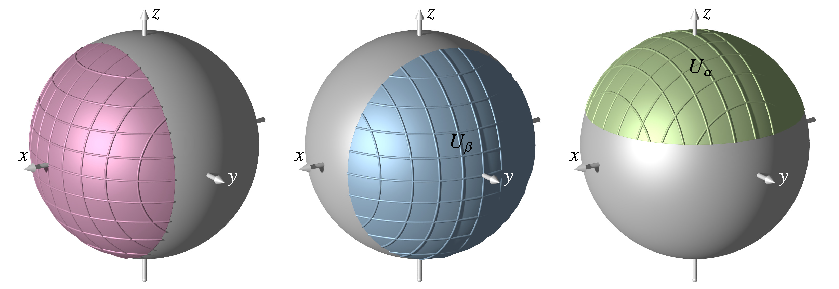
\includegraphics{chapters/030-gruppen/images/kugelkarten.pdf}
\caption{Drei verschiedene Karten auf einer Kugeloberfläche jeweils in
einer Umgebung der Schnittpunkte der Kugeloberfläche mit einer
Achse.
\label{buch:gruppen:gruppe:fig:kugelkarten}}
\end{figure}
Die Menge $S^2 = \{(x,y,z)\mid x^2+y^2+z^2=1\}$ ist eine Kugeloberfläche.
In der Umgebung $U_\alpha = \{(x,y,z)\in S^2\mid x^2+y^2<0.9\wedge z>0\}$
des Nordpoles ist die Abbildung
\[
\varphi_\alpha
\colon
U_\alpha
:
(x,y,z)\mapsto (x,y)
\]
eine gute Karte, sie deckt aber alle anderen Pole überhaupt nicht ab.
In der Umgebung $U_\beta = \{(x,y,z)\in S^2\mid x^2+z^2<0.9\wedge y>0\}$
des Punktes $(0,1,0)$ ist die Abbildung
\[
\varphi_\beta
\colon
U_\beta
:
(x,y,z)\mapsto (x,z)
\]
dagegen eine gute Karte.
So kann für jeden Pol eine Karte gefunden werden, die in 
Abbildung~\ref{buch:gruppen:gruppe:def:karte} dargestellt sind.
\end{beispiel}

Das Beispiel zeigt, dass die vollständige Beschreibung einer Menge
eine Vielzahl von Karten benötigen kann.
Aus den Koordinatenfunktionen werden dann andere Eigenschaften der
Menge abgeleietet.
Dies kann jedoch nur funktionieren, wenn im Überschneidungsbereich
zweier Koordinatensysteme, die gleichen Eigenschaften abgeleitet
werden können.
Im nächsten Abschnitt wird genau dieses Problem für die
Charakterisierung der Differenzierbarkeit von Funktionen auf der
Menge adressiert.

%
% Ableitungen
%
\subsubsection{Ableitungen}
\begin{figure}
\centering
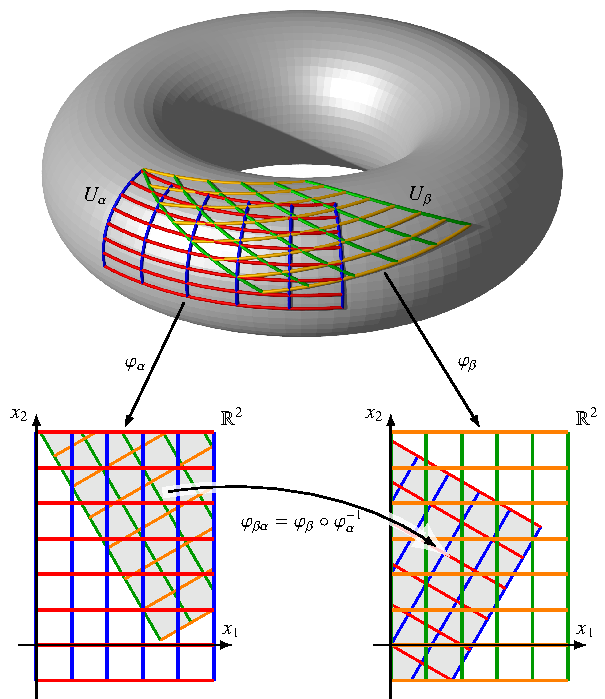
\includegraphics{chapters/030-gruppen/images/karten.pdf}
\caption{Kartenwechsel für zwei Karten auf einem Torus
\label{buch:gruppen:gruppe:fig:kartenwechsel}}
\end{figure}
Die Karten sollen der Menge $M$ ein Koordinatensystem geben, mit dem
man Ableitungen von Funktionen definieren kann.
Dazu ist notwendig, dass verschiedene Karten auf die gleiche
Ableitung führen.
Seien $x_i$ und $y_i$ Koordinaten für eine offene Teilmenge von $M$,
und $f$ eine Funktionen auf $M$.
In dieser Menge können die Koordinaten $x_i$ als Funktionen der 
Koordinaten $y_k$ in der Form $x_i(y_1,\dots,y_k)$ schreiben.
Ebenso kann man $f$ durch die Koordinaten $x_i$ ausdrücken, dies
schreiben wir als $f(x_1,\dots,x_n)$, oder durch die Koordinaten $y_i$,
dies schreiben wir als $f(y_1,\dots,y_n)$.
Die Ableitung der Funktion $f$ nach den Koordinaten $y_i$ muss nach
der Kettenregel
\begin{equation}
\frac{\partial f}{\partial y_i}
=
\sum_{k=1}^n
\frac{\partial f}{\partial x_k} \frac{\partial x_k}{\partial y_i}
\label{buch:gruppen:gruppe:eqn:kettenregel}
\end{equation}
auch durch die Ableitungen von $f$ nach den Koordinaten $y_i$
ausgedrückt werden können.
Die Formel~\ref{buch:gruppen:gruppe:eqn:kettenregel} ist aber nur sinnvoll,
wenn die Ableitungen $\partial x_k/\partial y_i$ alle existieren.
Die Kartenwelchselabbildung $y\mapsto x$ muss also differenzierbar sein.
Die Koordinatenumrechnung zwischen zwei Karten müssen also differenzierbare
Abbildungen sein.

Seien also
$\varphi_\alpha\colon U_\alpha \to \mathbb{R}^n$
und
$\varphi_\beta\colon U_\beta \to \mathbb{R}^n$
zwei Karten, deren Definitionsbereiche $U_\alpha$ und $U_\beta$ sich
schneiden.
Sie statten also beide die Menge $U_{\alpha\beta}=U_\alpha\cap U_\beta$
mit einem Koordinatensystem aus.
Die Koordinatenwechselabbildung
\[
\varphi_{\beta\alpha}
=
\varphi_\beta
\circ
\varphi_\alpha^{-1}
\colon
\varphi_\alpha(U_\alpha\cap U_\beta)
\to
\varphi_\beta(U_\alpha\cap U_\beta)
\]
ist eine Abbildung zwischen offenen Teilmengen von $\mathbb{R}^n$.
Man sagt, der Kartenwechsel ist differenzierbar, wenn $\varphi_{\beta\alpha}$
differenzierbar ist.
Der Kartenwechsel in der umgekehrten Richtung ist $\varphi_{\alpha\beta}$.

\begin{definition}
\label{buch:gruppen:gruppe:def:atlas}
Ein {\em differenzierbarer Atlas} von $M$ ist eine Menge von Karten derart,
dass alle Kartenwechselabbildungen differenzierbar sind.
\end{definition}

\begin{definition}
\label{buch:gruppen:gruppe:def:diffman}
Eine {\em differenzierbare Mannigfaltigkeit} ist eine Menge $M$ mit einem
differenzierbaren Atlas derart, dass jeder Punkt von $M$ im
Definitionsgebiet mindestens einer Karte liegt.
\end{definition}

Eine differenzierbare Mannigfaltigkeit ist also eine Menge, die in
einer Umgebung jedes Punktes mit mindestens einem Koordinatensystem
ausgestattet werden kann auf eine Art, dass die Umrechnung zwischen
verschiedenen Koordinatensystemen immer differenzierbar ist.

\begin{beispiel}
Die reelle Achse $\mathbb{R}$ ist eine differenzierbare Mannigfaltigkeit,
sie lässt sich mit einer einzigen Karte parametrisieren.
\end{beispiel}

\begin{beispiel}
Die Kreislinie $S^1$ in der komplexen Ebene ist eine differenzierbare
Mannigfaltigkeit, Karten können wie folgt konstruiert werden.
Die Abbildung $\mathbb{R}\to S^1: x\mapsto e^{ix}$ bildet die ganze
reelle Achse auf die Kreislinie ab.
Die Abbildung ist allerdings nicht umkehrbar, weil $x$-Werte, die sich
um Vielfache von $2\pi$ unterscheiden, auf den gleichen Punkt in $S^1$
abgebildet werden.
Zu jedem Punkt $x\in\mathbb{R}$ gibt es aber ein Intervall
$U_x=(x-1,x+1)$, welches bijektiv auf eine Teilmenge von $S^1$
abgebildet wird.
Die Exponentialabbildung von $U_x\to S^1$ wie auch die Umkehrabbildung
von der Bildmenge zurück in $U_x$ sind stetig.
Die Koordinaten, die verschiedene solche Karten einem Punkt der Kreislinie
zuordnen können, unterscheiden sich immer um Vielfache von $2\pi$.
Die Koordinatenwechsel-Abbildung zwischen zwei Karten $U_x$ und $U_y$
sind also Abbildungen der Form $x\mapsto x+2\pi k$ mit $k\in\mathbb{Z}$,
also sicher differenzierbar.
Damit ist ein differenzierbarer Atlas für $S^1$ konstruiert, $S^1$
ist eine differenzierbare Mannigfaltigkeit.
\end{beispiel}

\begin{beispiel}
\begin{figure}
\centering
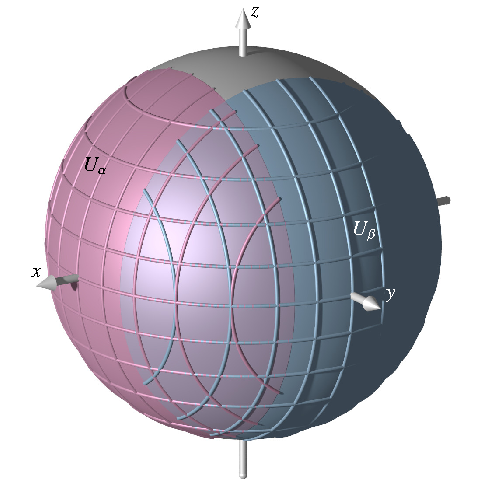
\includegraphics{chapters/030-gruppen/images/kugelschnitt.pdf}
\caption{Zwei Karten der Kugeloberfläche und deren Schnittbereich.
Differenzierbarkeit von Funktionen auf der Kugeloberfläche kann mit
Hilfe der Karten nur dann definiert werden, wenn die Kartenwechselabbildung
$\varphi_\alpha\circ\varphi_\beta^{-1}$ und
$\varphi_\beta\circ\varphi_\alpha^{-1}$ differenzierbare Abbildungen
zwischen offenen Mengen in $\mathbb{R}^n$ sind.
\label{buch:gruppen:gruppe:fig:kugelkartenwechsel}}
\end{figure}
Die Ableitung von Funktionen auf einer Kugeloberfläche muss auf 
die Beschreibung der Funktion in einer Karte mit Hilfe der dortigen
Koordinaten zurückführen.
Dazu ist notwendig, dass die Kartenwelchselabbildungen differenzierbar
sind.
Für die in Beispiel~\ref{buch:gruppen:gruppe:bsp:kugel} gezeigten
Karten auf der Kugeloberfläche ist dies leicht nachzurechnen.
Das in Abbildung~\ref{buch:gruppen:gruppe:fig:kugelkartenwechsel}
hat die Kartenwechselfunktion
\[
\varphi_\beta
\circ
\varphi_\alpha^{-1}
\colon
\varphi_\alpha(U_\alpha\cap U_\beta)
\to
\varphi_\beta(U_\alpha\cap U_\beta)
:
(x,z) \mapsto (x,\!\sqrt{1-x^2-z^2}),
\]
die offensichtlich differenzierbar ist, solange $x^2+z^2<1$ ist.
\end{beispiel}

%
% Differenzierbare Abbildungen
%
\subsubsection{Differenzierbare Abbildungen}
Ein differenzierbarer Atlas erlaubt jetzt auch Abbildungen zwischen
verschiedenen Mannigfaltigkeiten zu definieren.
Sind $M$ und $N$ differenzierbare Mannigfaltigkeiten der Dimension $m$
bzw.~$n$ und $f\colon M\to N$ eine Abbildung.
Ist $x\in M$ ein Punkt in $M$, dann gibt es eine Karte
$\varphi_\alpha\colon U_\alpha\to\mathbb{R}^m$ mit $x\in U_\alpha$
und eine Karten $\psi_\gamma\colon V_\gamma\to\mathbb{R}^n$ mit
$f(x)\in V_\gamma$.
In einer Umgebung von $\varphi_\alpha(x)$ kann die Abbildung $f$
in den Koordinaten als
\[
f_{\gamma,\alpha}
=
\psi_\gamma\circ f \circ \varphi_\alpha^{-1}
\]
geschrieben werden.
Als Abbildung einer offenen Menge in $\mathbb{R}^m$ in eine offene
Menge in $\mathbb{R}^n$ ist wohldefiniert, was es heisst, dass die
Abbildung differenzierbar ist.

Wählt man andere Karten $\varphi_\beta\colon U_\beta\to\mathbb{R}^n$
und $\psi_\delta\colon V_\delta\to\mathbb{R}^n$, die ebenfalls
das Urbild $x\in U_\beta$ und das Bild $f(x)\in V_\delta$ enthalten,
dann lässt sich die Funktion auch durch die neuen Koordinaten
\[
f_{\delta,\beta}
=
\psi_\delta\colon \circ f \circ\varphi_\beta^{-1}
\]
ausdrücken.
Natürlich muss auch $f_{\delta,\beta}$ differenuzierbar sein.
Diese beiden Arten, die Ableitung zu definieren, sind miteinander
konsistent, weil für die Zusammensetzung
\[
f_{\gamma,\alpha}
=
\psi_\gamma\circ\psi_\delta^{-1}
\circ
f_{\delta,\beta}
\circ
\varphi_\beta\circ\varphi_\alpha^{-1}
=
\psi_{\gamma\delta}
\circ
f_{\delta,\beta}
\circ
\varphi_{\beta\alpha}
\]
die Kettenregel gilt und die Kartenwechselabbildungen $\varphi_{\beta\alpha}$
und $\psi_{\gamma\delta}$ differenzierbar sind.

%
% Lie-Gruppen
%
\subsubsection{Lie-Gruppen}
Die Gruppen $S^1$ war als differenzierbare Mannigfaltigkeit erkannt
worden.
Damit die Struktur der Gruppe und die differenzierbare Struktur sinnvoll
miteinander verwendet werden können ist notwendig, dass die
Verknüpfungsabbildung $(x,y)\mapsto xy$ und die Umkehrabbildung
$x\mapsto x^{-1}$ nicht nur stetig, sondern sogar differenzierbar sind.

\begin{definition}
\label{buch:gruppen:gruppe:def:liegruppe}
Eine Lie-Gruppe ist eine Gruppe, die gleichzeitig eine differenzierbare
Mannigfaltigkeit ist derart, dass die Gruppenoperation
$G\times G\to G:(x,y)\mapsto xy$
und die Invertierung $G\to G: x\mapsto x^{-1}$ differenzierbare Abbildungen
sind.
\end{definition}

In den für die Gruppe $S^1$ konstruierten Karten ist die Verknüpfung die
Addition von Koordinaten und die Invertierung ist der Vorzeichenwechsel.
Beide sind differenzierbar, daher ist $S^1$ eine Lie-Gruppe.

%
% Koordinatensysteme auf Matrizengruppen
%
\subsubsection{Koordinatensysteme auf Matrizengruppen}
Die allgemeine lineare Gruppe $\operatorname{GL}_n(\mathbb{R})$
ist eine offene Teilmenge von $\mathbb{R}^{n\times n}$ ist.
Die Matrixelemente $a_{ik}$ sind daher auf natürliche Weise ein
Koordinatensystem auf der Gruppe $\operatorname{GL}_n(\mathbb{R})$.
Die Gruppenoperationen lassen sich als Summen von Produkten von
Matrixelementen schreiben.
Mit den Matrixelementen als Koordinaten folgt unmittelbar, dass
die Gruppenoperationen differenzierbare Abbildungen sind.

Alle anderen Matrizengruppen sind Teilmengen von
$\operatorname{GL}_n(\mathbb{R})$ niedrigerer Dimension.
Zum Beispiel besteht die Gruppe $\operatorname{SL}_n(\mathbb{R})$
aus den Matrizen mit Determinante $1$, der $(n^2-1)$-dimensionalen
Teilmenge von $\operatorname{GL}_n(\mathbb{R})$ bestehend aus
den Nullstellen der Gleichung $\det(A)-1=0$.
Die Gruppe $\operatorname{SO}(n)$ besteht aus den Matrizen, die
zusätzlich $A^tA=I$ erfüllen.
Da $A^tA$ eine symmetrische Matrix ist, sind dies
$n(n+1)/2$ unabhängige Bedinungen.
Da daraus auch $\det A=\pm$ folgt, ist die $n(n-1)/2$ Dimension der Gruppe
$\operatorname{SO}(n)$, denn
\[
n^2 - \frac{n(n+1)}2
=
\frac{2n^2-n^2-n}{2}
=
\frac{n^2-n}2
=
\frac{n(n-1)}2.
\]
Da diese Einschränkungen ausserdem differenzierbar sind und in der
Einheitsmatrix keine Singularitäten haben, kann man davon ausgehen,
dass diese Teilmengen Untermannigfaltigkeiten sind.

Kann man auf kanonische Art Karten für die Matrizengruppen
konstruieren?
Die Matrixform der Rodrigues-Formel (\cite[p.~438]{buch:linalg})
beschreibt Drehungen des dreidimensionalen Raumes um die Achse mit
Richtung des Einheitsvektors $\vec{u}$ und um den Drehwinkel $\alpha$a
durch die Matrix
\[
D_{\vec{u},\alpha}
=
\begin{pmatrix}
 1-(1-c)(1-u_1^2) & -su_3+(1-c)u_1u_2 &  su_2+(1-c)u_1u_3 \\
 su_3+(1-c)u_1u_2 &  1-(1-c)(1-u_2^2) & -su_1+(1-c)u_2u_3 \\
-su_2+(1-c)u_1u_3 &  su_1+(1-c)u_2u_3 &  1-(1-c)(1-u_3^2) 
\end{pmatrix}
\]
beschrieben werden kann.
Der Vektor $\vec{u}$ ist ein Einheitsvektor und daher $\vec{u}\in S^2$
ein Punkt auf einer Kugel.
Wählt man auf der Kugel eine Karte, kann man daraus zusammen mit den
Drehwinkeln eine Karte für die Drehmatrizen konstruieren.
Dies zeigt, dass $\operatorname{SO}(3)$ eine differenzierbare
Mannigfaltigkeit ist.

Die Konstruktion des vorangeangenen Absatzes ist nicht direkt
auf andere Matrizengruppen verallgemeinerbar.
Man kann aber zeigen, dass in einer Umgebung der Einheitsmatrix
sich die Matrizen einer Matrizengruppe mit Hilfe der Exponentialreihe
schreiben lassen (siehe auch \cite[Abschnitt~9.4.4]{buch:linalg}).
Zum Beispiel sind die Matrizen $A\in \operatorname{SL}_n(\mathbb{R})$
in einer Umgebung von $I$ von der Form
\(
e^U
\),
wobei
die  Matrix $U$ Spur $\operatorname{tr}{U}=0$ haben muss.
Die Menge der Matrizen mit Spur $0$ ist eine $(n^2-1)$-dimensionale
Teilmenge von $M_{n}(\mathbb{R})$.
Die Umkehrabbildung der Exponentialabbildung kann daher als Karte
in einer Umgebung von $I$ dienen.

Ganz allgemein ist die Exponentialabbildung immer eine lokal
invertierbare Abbildung von der Lie-Algebra einer Matrizengruppe
in die Lie-Gruppe.
Da die Lie-Algebra ein $\mathbb{R}$-Vektorraum ist, kann eine
lokale Umkehrabbildung um die Einheitsmatrix $I$ als Karte mit
Werten in der Lie-Algebra dienen.
Für die Gruppe $\operatorname{SO}(3)$ zum Beispiel besteht die
Lie-Algebra aus antisymmetrischen Matrizen, also Matrizen
der Form
\[
U
=
\begin{pmatrix}
  0  & -u_3 &  u_2 \\
 u_3 &   0  & -u_1 \\
-u_2 &  u_1 &   0
\end{pmatrix}.
\]
Die Exponentialabbildung ordnet der Matrix $U$ die Matrix $e^U$
zu, die nach der Exponentialform der Rodrigues-Formel 
(\cite[p.~483]{buch:linalg}) die Drehmatrix der Drehung um die
Achse mit Richtung $\vec{u}^0$ und mit Drehwinkel $\alpha=|\vec{u}|$
ist, wobei $\vec{u}$ der Vektor mit den Komponenten $u_1$, $u_2$ und
$u_3$ ist.
Das Tripel $(u_1,u_2,u_3)$ bildet also ein gutes Koordinatensystem
für eine Umgebung der Einheitsmatrix in der Gruppe $\operatorname{SO}(3)$.

Die aus der Lie-Algebra konstruierten Karten zeigen noch mehr.
Da die Exponentialabbildung beliebig oft differenzierbar ist und die
Matrixmultiplikation durch Polynome höchstens zweiten Grades in
den Matrixelementen ausgedrückt werden kann, sind die Koordinatenwechsel
immer beliebig oft differenzierbar.
Die Matrizengruppen sind also sogar beliebig oft differenzierbare
Mannigfaltiketen. 
Es ist daher zulässig, sich für die Zwecke der nachfolgenden Diskussionen
immer auf beliebig oft differenzierbare Funktionen einzuschränken.
Andere, weniger oft differenzierbare Funktionen können durch
solche Funktionen beliebig genau approximiert werden.

